%%%%%%%%%%%%%%%%%%%%%%%%%%%%%%%%%%%%%%%%%%%%%%%%%%%%%%%%%%%%%%%%%%%%%%%%%%%%%%%
\section{SuPerHomog\'{e}n\'{e}isation Factors}
\label{sec:sph}
%%%%%%%%%%%%%%%%%%%%%%%%%%%%%%%%%%%%%%%%%%%%%%%%%%%%%%%%%%%%%%%%%%%%%%%%%%%%%%%

Hmm \cite{askew1972moc} \cite{hebert2005ribon}, \cite{hebert1993consistent} \cite{hebert1997advances}

-angular dependent total MGXS only true solution

\begin{figure}[h!]
\centering
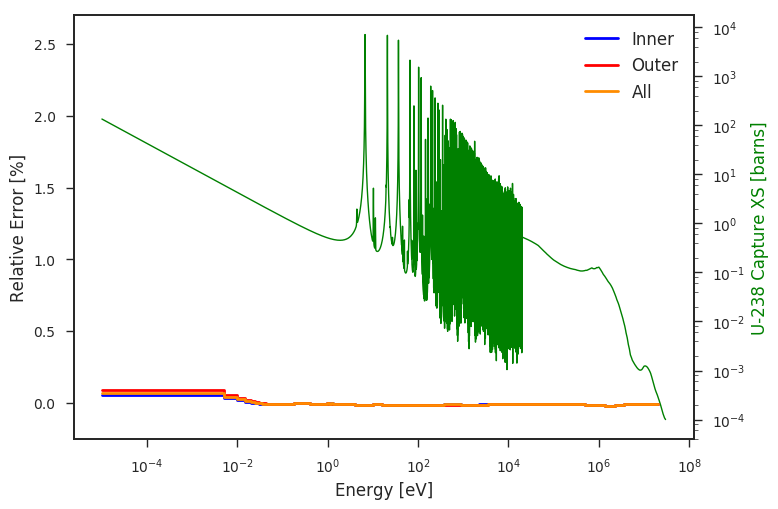
\includegraphics[width=\linewidth]{figures/rel-err-inner-outer-sph}
\caption{The energy-dependent relative error of the OpenMOC scalar flux computed with SPH-corrected MGXS with respect to the reference OpenMC flux for the innermost, outermost and all FSRs.}
\label{fig:rel-err-energy-sph}
\end{figure}


%%%%%%%%%%%%%%%%%%%%%%%%%%%%%%%%%%%%%%%%%%%%%%%%%%%%%%%%%%%%%%%%%%%%%%%%%%%%%%%
\subsection{Overview}
\label{subsec:sph-overview}

The SPH algorithm enforces reaction rate preservation between a reference fine-mesh transport problem and a corresponding coarse mesh transport or diffusion problem in energy and space. SPH factors have traditionally been applied to spatially-homogenized few-group MGXS for coarse mesh diffusion applications. However, this section will introduce SPH factors to enforce equivalence between continuous energy Monte Carlo and deterministic multi-group transport methods. 

The SPH scheme postulates the existence of a set of factors $\mu_{k,g}$ for each spatial zone $k$ and energy group $g$ which force the streaming and collision terms in the transport equation to balance with a fixed source $Q_{k,g}$:

\begin{dmath}
\label{eqn:chap6-sph-transport-eqn}
\mathbf{\Omega} \cdot \nabla \psi_{g}(\mathbf{r},\mathbf{\Omega}) + \mu_{k,g}\Sigma_{t,k,g}\psi_{g}(\mathbf{r},\mathbf{\Omega}) = Q_{k,g}(\mathbf{\Omega})
\end{dmath}

\noindent In this equation, the SPH factors are applied to correct the total MGXS in each region and group. The fixed source $Q_{k,g}$ is computed from the reference fine-mesh solution. In this case,  the fixed source is treated as the sum of scattering and fission production sources in each energy group and spatial zone. For example, continuous energy Monte Carlo can be used to compute reference multi-group fluxes and MGXS, which are then combined to compute an isotropic source as follows:

\begin{dmath}
\label{eqn:chap6-sph-source}
Q_{k,g}(\mathbf{\Omega}) = \frac{1}{4\pi} \sum_{g'=1}^{G} \Sigma_{s,k,g' \rightarrow g}\phi_{k,g'} + \frac{\chi_{k,g}}{4\pi k_{eff}}\sum_{g'=1}^{G} \nu\Sigma_{f,k,g'}\phi_{k,g'}
\end{dmath}

\noindent Given the fixed source and total MGXS from MC, Eqn.~\ref{eqn:chap6-sph-transport-eqn} may be solved using any multi-group transport method, such as MOC. The challenge is to devise estimates to the true SPH factors $\mu_{k,g}$ which adequately preserve reaction rates. The following section describes the iterative scheme used to estimate SPH factors.


%%%%%%%%%%%%%%%%%%%%%%%%%%%%%%%%%%%%%%%%%%%%%%%%%%%%%%%%%%%%%%%%%%%%%%%%%%%%%%%
\subsection{Algorithm}
\label{sec:sph-algorithm}

An iterative algorithm is used to estimate SPH factors from a series of multi-group fixed source calculations. First, the estimates $\mu_{k,g}^{(n)}$ at iteration $n$ to the true SPH factors $\mu_{k,g}$ are introduced as a correction factor for the total cross section in Eqn.~\ref{eqn:chap6-sph-transport-eqn}:

\begin{dmath}
\label{eqn:chap6-sph-transport-eqn-iterate}
\mathbf{\Omega} \cdot \nabla \psi_{g}^{(n)}(\mathbf{r},\mathbf{\Omega}) + \mu_{k,g}^{(n-1)}\Sigma_{t,k,g}\psi_{g}^{(n)}(\mathbf{r},\mathbf{\Omega}) = Q_{k,g}(\mathbf{\Omega})
\end{dmath}

\noindent A multi-group transport code (such as OpenMOC) may be used to solve Eqn.~\ref{eqn:chap6-sph-transport-eqn-iterate} with angular and volume integration to compute the scalar flux distribution. The SPH factor estimates $\mu_{k,g}^{(n)}$ are found from the ratio of the reference Monte Carlo scalar flux $\phi_{k,g}^{MC}$ to the flux $\phi_{k,g}^{(n)}$ computed from the fixed source calculation at iteration $n$,

\begin{equation}
\label{eqn:chap6-sph-update}
\mu_{k,g}^{(n)} = \frac{\phi_{k,g}^{MC}}{\phi_{k,g}^{(n)}}
\end{equation}

\noindent where the factors are initialized to unity on the first iteration:

\begin{dmath}
\label{eqn:chap6-sph-initial}
\mu_{k,g}^{(0)} = 1
\end{dmath}

The SPH factors are used to find a total MGXS which forces neutron balance in Eqn.~\ref{eqn:chap6-sph-transport-eqn-iterate}. The initial total MGXS $\Sigma_{t,k,g}^{(0)}$ is computed from the reference MC flux and total reaction rate tallies. The SPH factors are then used to obtain a corrected total MGXS $\Sigma_{t,k,g}^{(n)}$ on each iteration:

\begin{dmath}
\label{eqn:chap6-sph-update-sigt}
\Sigma_{t,k,g}^{(n)} = \mu_{k,g}^{(n-1)}\Sigma_{t,k,g}^{(0)}
\end{dmath}

The series of fixed source problems defined by Eqn.~\ref{eqn:chap6-sph-transport-eqn-iterate} are solved until the SPH factors converge. A common convergence criterion is the maximum relative absolute deviation across energy groups and spatial zones:

\begin{dmath}
\label{eqn:chap6-sph-residual}
res = \max_{k,g} \left|\frac{\mu_{k,g}^{(n)} - \mu_{k,g}^{(n-1)}}{\mu_{k,g}^{(n-1)}}\right|
\end{dmath}

\noindent A residual of 10$^{-7}$ can typically be achieved with twenty or fewer iterations.

The scattering matrix $\Sigma_{s,k,g'\rightarrow g}$ and fission production cross section $\nu\Sigma_{f,k,g}$ are used to compute the reference fixed source in Eqn.~\ref{eqn:chap6-sph-source}, but are not needed in the iterative scheme defined in Eqn.~\ref{eqn:chap6-sph-transport-eqn-iterate}. However, in the context of this thesis, SPH factors are computed to preserve reaction rates in subsequent eigenvalue calculations. Therefore, the SPH factors must be applied to the scattering matrix and fission production cross sections to produce a fully-corrected MGXS library:

\begin{dmath}
\label{eqn:chap6-sph-update-sigs}
\Sigma_{s,k,g'\rightarrow g}^{(n)} = \mu_{k,g}^{(n-1)}\Sigma_{s,k,g'\rightarrow g}^{(0)}
\end{dmath}

\begin{dmath}
\label{eqn:chap6-sph-update-nusigf}
\nu\Sigma_{f,k,g}^{(n)} = \mu_{k,g}^{(n-1)}\nu\Sigma_{f,k,g}^{(0)}
\end{dmath}

It should be noted that although the SPH-corrected MGXS are defined to preserve reaction rates, they will not preserve the group-wise scalar flux. However, the angular or scalar flux may be easily recovered from the fluxes $\tilde{\psi}_{k,g}$ and $\tilde{\phi}_{k,g}$ computed with the SPH-corrected MGXS in an eigenvalue or fixed source calculation:

\begin{dmath}
\label{eqn:chap6-sph-update-angular-flux}
\psi_{k,g} = \mu_{k,g}\tilde{\psi}_{k,g}
\end{dmath}

\begin{dmath}
\label{eqn:chap6-sph-update-scalar-flux}
\phi_{k,g}^{(n)} = \mu_{k,g}\tilde{\phi}_{k,g}
\end{dmath}

The SPH iteration algorithm described here is summarized in Alg.~\ref{alg:chap6-sph}. It should be noted that as presently posed, there is no unique solution to the set of SPH factors which preserve reaction rates. A unique solution may be found by forcing the factors to be unity in non-fissile zones (\textit{e.g.}, moderator, clad and gap)\footnote{A formulation of the SPH algorithm which corrected MGXS in both fissile and non-fissile zones was also implemented. This formulation introduced an outer loop over each spatial zone in Alg.~\ref{alg:chap6-sph}. The scheme is not presented here since it was unstable and the SPH factors diverged after a few outer iterations. Future work may develop a more rigorous approach to preserve reaction rates in each spatial zone.}. This approach is motivated by the fact that resonances which lead to self-shielding errors -- such as the U-238 capture resonances studied in Sec.~\ref{subsec:chap2-angle} -- are generally from isotopes in the fuel. However, the reaction rates in non-fissile zones will not be preserved since the MGXS in these zones remain uncorrected, but these errors are likely dominated by those in the fuel as was shown for the PWR benchmarks in Sec.~\ref{subsec:chap5-diagnosis-rxn-rates}.

\begin{algorithm}[h]
\caption{SPH Factor Algorithm}
\label{alg:chap6-sph}
\begin{algorithmic}[1]
  \State Initialize $\Sigma_{t,k,g}^{(0)}$, $\Sigma_{s,k,g'\rightarrow g}^{(0)}$, $\nu\Sigma_{f,k,g}^{(0)}$, and $\chi_{k,g}^{(0)}$ from MC tallies \Comment{Tab.~\ref{table:chap3-tally-types}}
  \State Compute $Q_{k,g}$ from MC flux and MGXS \Comment{Eqn.~\ref{eqn:chap6-sph-source}}
  \State Initialize $\mu_{k,g}^{(0)}$ to unity
  \While{SPH factor residuals are not converged}
    \State Update $\Sigma_{t,k,g}^{(n)}$ with SPH factors \Comment{Eqn.~\ref{eqn:chap6-sph-update-sigt}}
    \State Solve fixed source transport problem\footnotemark \Comment{Eqn.~\ref{eqn:chap6-sph-transport-eqn-iterate}}
    \State Compute new SPH factors $\mu_{k,g}^{(n)}$ \Comment{Eqn.~\ref{eqn:chap6-sph-update}}
    \State Compute SPH factor residuals \Comment{Eqn.~\ref{eqn:chap6-sph-residual}}
  \EndWhile
  \State Compute final MGXS with SPH factors \Comment{Eqns.~\ref{eqn:chap6-sph-update-sigt},~\ref{eqn:chap6-sph-update-sigs},~\ref{eqn:chap6-sph-update-nusigf}}
\end{algorithmic}
\end{algorithm}

\footnotetext{A series of $G$ independent fixed source problems may be solved for each of the $G$ groups. Alternatively, a single fixed source problem may simultaneously solve for all $G$ groups, as is done in OpenMOC.}


%%%%%%%%%%%%%%%%%%%%%%%%%%%%%%%%%%%%%%%%%%%%%%%%%%%%%%%%%%%%%%%%%%%%%%%%%%%%%%%
\subsection{Results}
\label{sec:sph-results}

-show plot of flux errors with SPH across fuel pin
-results for a 2D fuel pin with MGXS tallied by FSR


\begin{table}[h!]
  \centering
  \caption{The eigenvalue bias with SPH-corrected MGXS.}
  \label{table:keff-bias-sph} 
  \begin{tabular}{c S[table-format=6.1] S[table-format=6.1] S[table-format=6.1]}
  \toprule
  & \multicolumn{3}{c}{{\bf FSR Discretization}} \\
  \midrule
  \multicolumn{1}{c}{{\bf \# Groups}} &
  {\bf 1$\times$} & {\bf 4$\times$} & {\bf 16$\times$} \\
  \midrule
1 & 19 & -18 & -14 \\
2 & 25 & -14 & -6 \\
4 & 7 & 2 & 1 \\
8 & 4 & -0 & 2 \\
16 & 5 & 0 & 4 \\
25 & 5 & 2 & -1 \\
40 & 4 & 3 & -2 \\
70 & 4 & 2 & -3 \\
  \bottomrule
\end{tabular}
\end{table}